\documentclass{beamer}
\usepackage{times, amsthm, amsmath, amssymb, cancel, changepage, graphicx, lipsum, fancyhdr, mathabx, enumitem,caption, subcaption}
\usetheme{CambridgeUS}
\usecolortheme{seagull}
\usefonttheme{serif}
\definecolor{navy}{RGB}{0, 0, 128} 
\setbeamercolor{frametitle}{fg=navy}
\setbeamercolor{title}{fg=navy}

\title{\textbf{Lecture 11: Multiple Integration II}}
\date{October 1, 2019}

\begin{document}
	
\frame{\titlepage}


\begin{frame}
\frametitle{\textbf{Double Integration with General Region}}
\begin{figure}
	\centering
	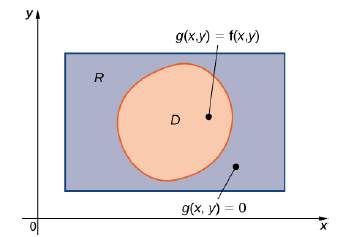
\includegraphics[height=.35\textheight]{DR.png}\\
	\hspace*{10pt}\hbox{\thinspace{\tiny\itshape math.libretexts.org}}
\end{figure}
If we want to integrate $f(x,y)$ over $D$, define a new function with domain $R$
$$F(x,y) = \begin{cases}
f(x,y) & \mbox{if }(x,y)\in D\\
0 & \mbox{otherwise}
\end{cases}$$
Then if $F$ is integrable over $R$, $f$ is integrable over $D$.
$$\iint\limits_{D} f(x,y)dA = \iint\limits_{D} F(x,y)dA$$
\end{frame}

\begin{frame}
\frametitle{Type I vs Type II Regions}
\begin{figure}
	
		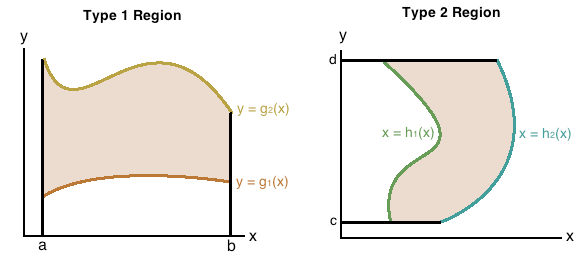
\includegraphics[width=.95\textwidth]{image001.png}
		\hspace*{10pt}\hbox{\thinspace{\tiny\itshape mathonline.wikidot.com}}
\end{figure}
\end{frame}


\begin{frame}
\frametitle{\textbf{Type I Region}}
A Type I region is defined as:
$$D = \{(x,y)| \,a \leq x \leq b, g_1(x) \leq y \leq g_2(x)\}$$
where $g_1$ and $g_2$ are continuous on $[a,b]$. Then
$$\iint\limits_{D} f(x,y)dA = \int_a^b \int_{g_1(x)}^{g_2(x)} f(x,y)dy\,dx$$
\vspace{12pt}
\textbf{Example:}
\begin{itemize}
	\item [(a)] Integrate $f(x,y) = x+2y$ on $D = \{(x,y)|-1\leq x \leq, 2x^2 \leq y \leq 1+x^2\}$
\end{itemize}
\end{frame}

\begin{frame}
\frametitle{\textbf{Type II Region}}
A Type II region is defined as:
$$D = \{(x,y)| \,h_1(y) \leq x \leq h_2(y), c \leq y \leq d\}$$
where $h_1$ and $h_2$ are continuous on $[c,d]$. Then
$$\iint\limits_{D} f(x,y)dA = \int_c^d \int_{h_1(y)}^{h_2(y)} f(x,y)dx\,dy$$
\vspace{12pt}

\textbf{Example:}

\begin{itemize}
	\item[(a)] Integrate $f(x,y) = xe^{y}$ on $D = \{(x,y)|\sqrt{y}\leq x \leq 1/2y, 0\leq y \leq 1 \}$.
\end{itemize}
\end{frame}

\begin{frame}
\frametitle{\textbf{The Approach I Use (An Aside)}}
In practice, you'll rarely have $D$  presented to you in a nice way that makes it obvious what type of region you're looking at. More often it looks like:\\
\vspace{12pt}
\begin{center}
	Integrate $f(x,y) = e^{x+y}$ over $y,x>0$ and $x>y$.
\end{center}
\vspace{12pt}
So you need to be able to tell from a graph how to set up your bounds. I typically use something called the "Rectangle and Line" method.\\
\vspace{12pt}
\textbf{Example:}
\begin{itemize}
	\item[(a)] Integrate $f(x,y) = 4xy$ on the trapezoid with corners at $(0,0)$, $(4,0)$, $(2,2)$, and $(4,2)$.
\end{itemize}
\end{frame}


\begin{frame}
\frametitle{\textbf{Several Examples}}

\begin{itemize}
	\item[(a)] Find the volume of the solid that lies under $f(x,y) = x^2+y^2$ and above region $D$ that is bounded by $x=y/2$ and $x=\sqrt{y}$
	\item[(b)] Integrate $f(x,y)=xy$ over the region bounded by $y=x-1$ and $y^2=2x+6$.
	\item[(c)] Integrate $f(x,y) = e^{y^2}$ where $y\leq1$, $y\geq x$, and $x\geq0$.
	\item[(d)] Integrate $f(x,y)=x^2+y^3$ over the region in the first quadrant bounded by $y=x^2$ and $x=y^4$.
\end{itemize}
\end{frame}

\end{document}
